\begin{frame}
    \frametitle{Cyclus vs. Unified Database: Major Isotopic Composition}
    \begin{figure}[htbp!]
        \begin{center}
          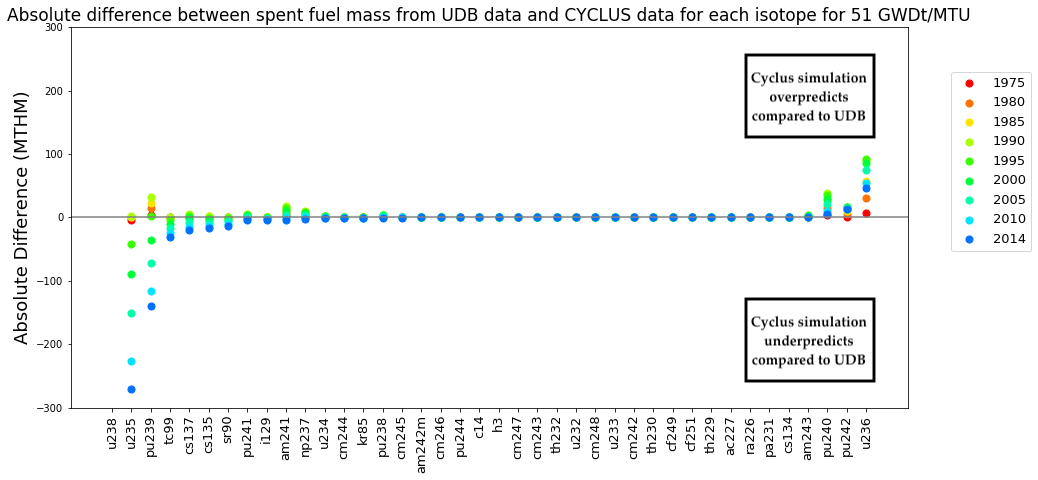
\includegraphics[height=5.3cm]{../figures/absolute_diff_all_51}
        \end{center}
              \caption{The absolute difference between cumulative spent fuel mass calculated by 
              Unified Database and \textsc{Cyclus} for each isotope. Spent fuel burnup of 51 GWD/MTU is used in the \textsc{Cyclus} simulation.
              Positive difference indicates \textsc{Cyclus}
              mass estimate is larger.}
        \label{fig:totalmass}
      \end{figure}
\end{frame}

\begin{frame}
    \frametitle{Cyclus vs. Unified Database: Major Isotopic Composition}
    \begin{figure}[htbp!]
        \begin{center}
          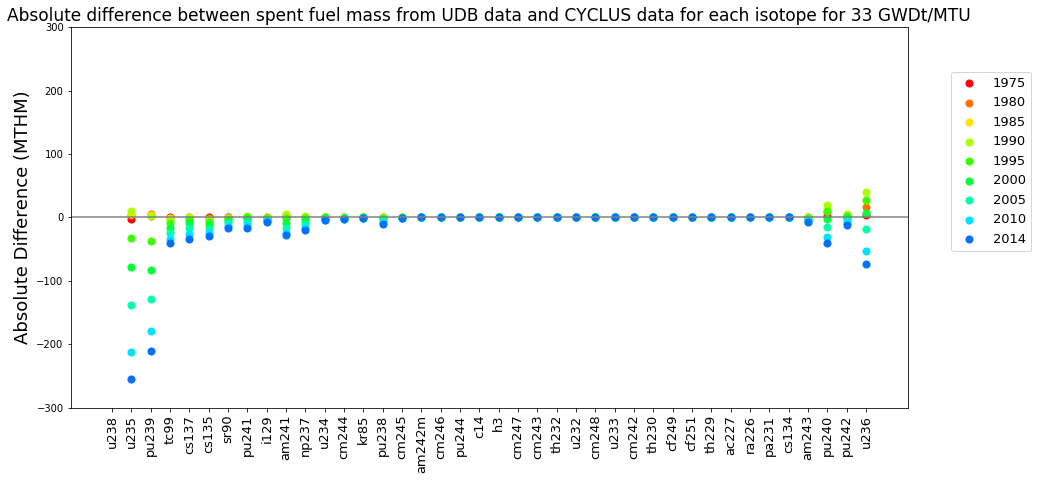
\includegraphics[height=5.3cm]{../figures/absolute_diff_all_33}
        \end{center}
        \caption{The absolute difference between cumulative spent fuel mass calculated by 
        Unified Database and \textsc{Cyclus} for each isotope. Spent fuel burnup of 33 GWD/MTU is used in the \textsc{Cyclus} simulation.
        Positive difference indicates \textsc{Cyclus}
        mass estimate is larger.}
        \label{fig:totalmass}
      \end{figure}
\end{frame}

\begin{frame}
    \frametitle{Burn up of Spent Nuclear Fuel}
    \begin{columns}
        \column[t]{5cm}
        \begin{figure}[htbp!]
        \begin{center}
        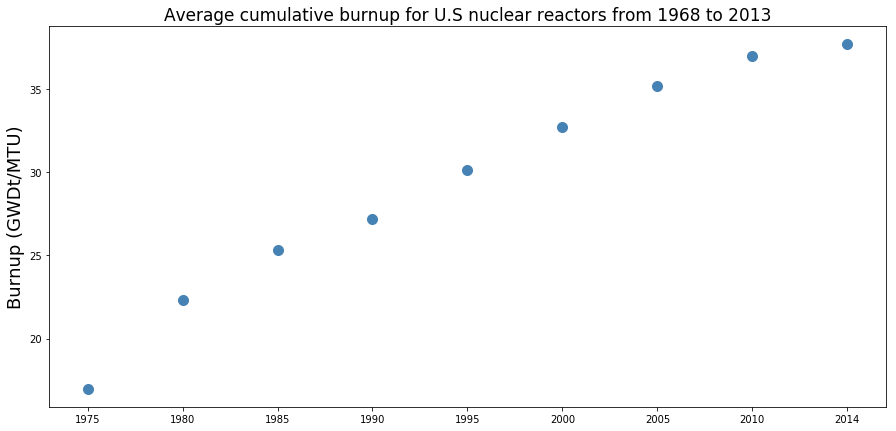
\includegraphics[height=2.8cm]{../figures/burn_up_real}
        \end{center}
        \caption{The average cumulative burnup for U.S. nuclear reactors
        from 1968 to 2013 \cite{eia_spent_2015}.}
        \end{figure}
        \column[t]{5cm}
        \begin{figure}[htbp!]
            \begin{center}
            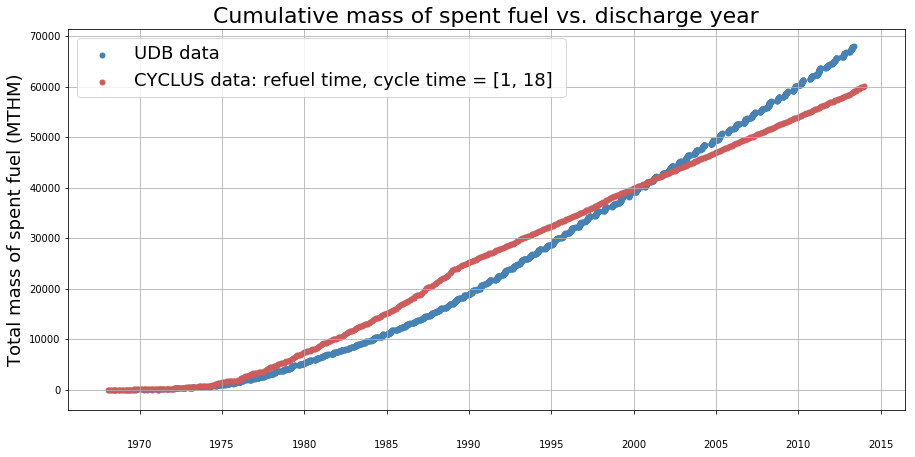
\includegraphics[height=2.8cm]{../figures/cumulative_mass_udb_cyclus}
            \end{center}
                \caption{The cumulative spent fuel mass against discharge time
                for Cyclus and Unified Database data from 1968 through 2013.}
          \label{fig:totalmass}
            \end{figure}
    \end{columns}
\end{frame}

\begin{frame}
    \frametitle{Cyclus vs. Unified Database: Major Isotopic Composition}
    \begin{figure}[htbp!]
        \begin{center}
          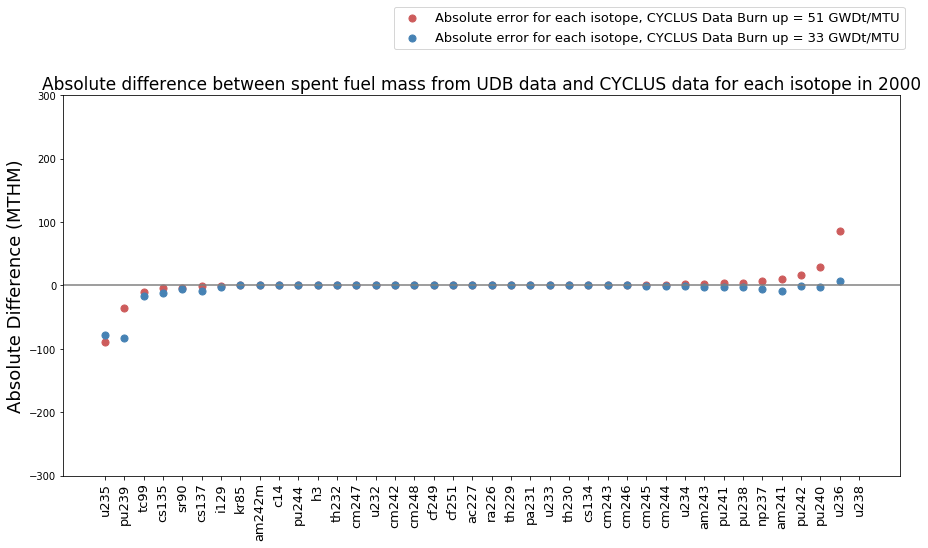
\includegraphics[height=6cm]{../figures/absolute_diff_2000}
        \end{center}
              \caption{The absolute difference between cumulative spent fuel mass calculated by 
              Unified Database and \textsc{Cyclus} for each isotope at year 2000. Positive difference indicates \textsc{Cyclus}
              mass estimate is larger.}
        \label{fig:totalmass}
      \end{figure}
\end{frame}

\begin{frame}
    \frametitle{Cyclus vs. Unified Database: Major Isotopic Composition}
    \begin{figure}[htbp!]
        \begin{center}
          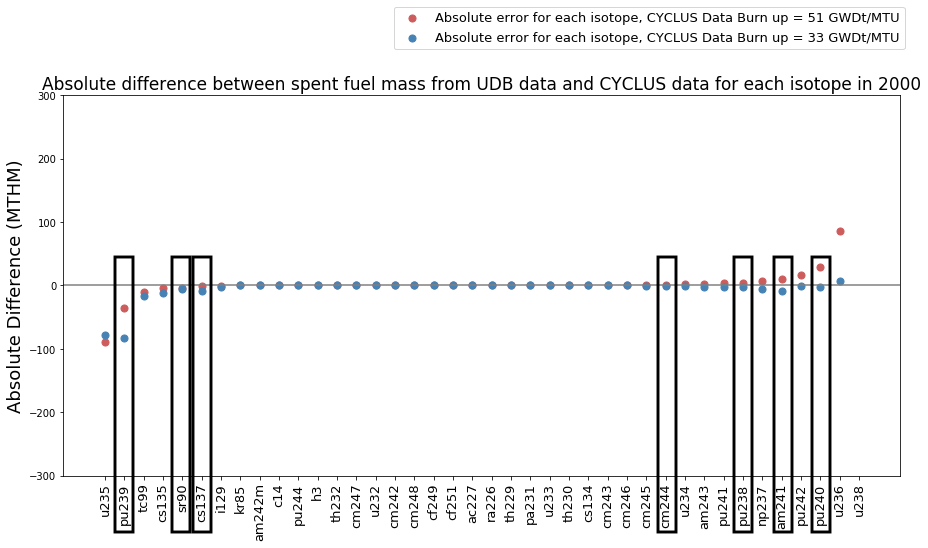
\includegraphics[height=6cm]{../figures/absolute_diff_2000_annotated}
        \end{center}
              \caption{The absolute difference between cumulative spent fuel mass calculated by 
              Unified Database and \textsc{Cyclus} for each isotope at year 2000. The boxed isotopes are the major decay heat contributors.}
        \label{fig:totalmass}
      \end{figure}
\end{frame}